Modern multimedia increasingly demands high flexibility and extensibility.
This is driven by a number of strong trends: device proliferation, new
sensors, new data types (e.g. sensor data, 3D, 360 degree video), multiple data
sources, live data, personalization, interactivity, responsiveness and multi-device 
support. On top of all this there are also rising expectations to UI
design, integration with social networks, and more.

In an attempt to meet such demands, new features have been added to media
frameworks allowing programmers to customize the media player to a larger
extent. For example, the Flash~\cite{flash} framework has grown increasingly
feature-rich over time, even having partially overlapping features with the
Web platform itself. Media Source Extensions (MSE)~\cite{mse} in HTML5
provide a way to manipulate the video stream client-side. It is also common
for media players to expose events and timed cues, allowing custom
functionality to be implemented in application code. The text track system of
HTML5 is an example of this. MPEG-4~\cite{mpeg4} adds support for
synchronization and composition of multiple media streams, including timed data
such as graphical objects (2D and 3D). In particular, the MPEG-4 Systems
part~\cite{mpeg4sys} defines an architecture for media clients (terminals)
integrating a variety of media formats, delivery methods, interactivity and
rendering.

In short, the need for extensibility has driven a development towards
standardization of new data formats and features, leading media players to
become increasingly sophisticated, yet also more complicated and heavyweight.
We call this the \emph{big player} approach to flexibility and extensibility in
multimedia.


\subsection{Multiple small players}

The motion model presents an attractive alternative to the big player
approach. The key idea is that a big player may be replaced by multiple
smaller players, with precisely synchronized playback. As illustrated in
Fig.~\ref{fig:motion-media}, the flexibility of the motion model allows a
variety of specialized media components to be coupled together, forming custom
and complex media experiences from simpler parts. We use the term Composite
Media~\cite{compositemedia} for media experiences built in this way.


\begin{figure}[h]
%\sidecaption
\centering
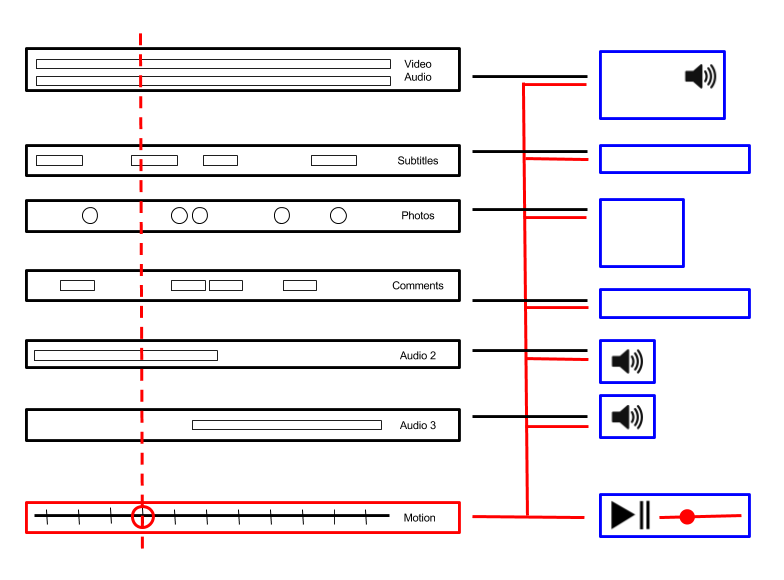
\includegraphics[scale=.4]{fig/motion-media.png}
\caption{A single media experience made from multiple media components (blue), possibly distributed across multiple devices. Each media component is connected to motion (red) and a source of timed data (black). There are different types of timed data: an AV container, a subtitle track, photos, comments and two extra audio tracks. The motion defines the timeline for the presentation, and timed data is mapped to this timeline by each media component. Since all the media components are connected to the same motion, they will operate in precise synchrony. One particular media component (bottom media element) provides interactive controls for the presentation, and connects only with motion.}
\label{fig:motion-media}
\end{figure}


\subsection{Dedicated media components}

The motion model typically encourages a pattern where each media
component is dedicated to solving a small and well defined challenge: Given
timed data and a motion, the media component must generate the correct presentation at
all times. Such custom media components are implemented in application code,
and an appropriate delivery method may be selected for the particular media
type and the task at hand. This way, application specific data formats may be
integrated into a presentation, as well as standardized formats. Importantly,
timed data sources may be dynamic and live, implying that presentations may
interact directly with live backend systems and update their presentations
during playback.

Media components may also be dedicated with respect to UI. For instance, a
single media component may implement interactive controls for the motion,
thereby relieving other media components from this added complexity. This
encourages a pattern where media components are designed for specific roles in
an application, e.g. controllers, viewers and editors, and combined to form
the full functionality. Of course, the fact that these media components are
independent may be hidden for end users with appropriate layout and styling,
giving the impression of a tightly integrated product. In any case, dedicated
media components may be reusable across different views, applications, devices
or data sets, as long as APIs to data model and motions remain unchanged.

\subsection{Flexible coupling}

The motion model allows modularity and flexibility by loose coupling of media
components. In fact, media components may be coupled only indirectly through
shared motions and shared data sources. This ensures that media components can
be added or removed dynamically during playback, or even fail, without
disrupting the rest of the presentation. This flexibility is also valuable in
development, as media components may be coded and tested in isolation or with
other components. New components may always be added without introducing any
additional increase in complexity, naturally supporting an incremental
development process. Also, the model does not impose restrictions on how
motions and timed data sources are connected with media components. A single
data source may be shared between multiple media components, or conversely, a
single media component may use multiple data sources. The same flexibility
goes for motions. There might be multiple aspects of timing and control in an
application, requiring multiple motions to be shared between media components.


\subsection{Client-side Synthesis}

Client-side synthesis is core design principle of the Web platform, and
central to key properties such as flexibility, extensibility, reusability and
scalability. This principle may now be fully exploited in the context of timed
media applications. With the motion model, timed media experiences
may be synthesised in real time within the browsing context (client-side), by
independent media components working directly on live data sources and
motions.

Interestingly, client-side synthesis is not the established approach to linear
media, not even in the Web context. With media frameworks such as Flash~\cite{flash} or
MPEG-4~\cite{mpeg4}, media is typically assembled in a media file or a media container, before
being downloaded or streamed to a client-side media player. Essentially, this is
server-side synthesis (and client-side playback). While server-side synthesis
may have certain advantages (e.g. robustness and simplicity), the
disadvantages are also evident. By assembling data within media files and container
formats, data is decoupled from its source and effectively flattened into an
immutable copy. Introduction of new media types may also be inconvenient, as this must be addressed through
standardization of new media and container formats, and support must be
implemented by media players. This may be a time-consuming process. That
said, server-side synthesis may still be an appropriate choice for a wide
range of media products.

Importantly though, in the motion model the choice between client-side 
synthesis and server-side synthesis is left to application programmers.
Established container-based media frameworks are still usable, provided only
that the framework can be integrated and controlled by external motion.
Ideally, this integration should be performed internally by the framework. If
this is done, frameworks can easily be used in conjunction with native media
elements, other frameworks or components that support external motion. If not,
integration may also be done externally, subject to the limitations of the
framework API. In any case, the motion model relieves media
frameworks from the challenge of doing everything, and highlights their value
as dedicated, reusable components.
